\section{Clase 1}
\subsection{Introducción: Estados microscópicos y entropía}
La termodinámica describe sistemas formados por una colección de elementos (muchos, $N\sim N_A=6.02\times 10^{23}$) en términos de variables que capturan el comportamiento colectivo del sistema. Por ejemplo, presión, volumen, energía, número de elementos potencial químico, entropía, temperatura.

En mecánica estadística, las variables se dividen en 2 tipos principales:
\begin{itemize}
	\item \textbf{Extensivas}: La magnitud es proporcional al tamaño o escala del sistema:
	\begin{itemize}
	\item Volúmen ($V$)
	\item Energía ($U$)
	\item Número de elementos ($N$)
	\item Entropía ($S$)
	\end{itemize}
	\item \textbf{Intensivas}: La magnitud no es proporcional al tamaño del sistema:
	\begin{itemize}
	\item Presión ($P$)
	\item Temperatura ($T$)
	\item Potencial químico ($\mu$)
	\end{itemize}
\end{itemize}

Estas variables corresponden a características (conceptos) atribuibles a los sistemas de forma colectiva (sin hacer mención a su estructura microscópica).

La mecánica estadística considera los microestados de un sistema dado por las \textbf{configuraciones cuánticas} en los que puede existir.

Una configuración microscópica (en términos de las cantidades termodinámicas) corresponde a michos microsestados diferentes, indistinguibles macroscópicamente. De lo anterior surgen las nociones de \textbf{degenerancia} y \textbf{entropía}.

La \textbf{entropía} mide el número de estados cuánticos accesibles a un sistema.

Es un \textit{postulado} que un sistema cerrado puede estar en cada microestado accesible con \textit{igual probabilidad}.

Dado $\Omega$ estados accesibles, la entropía $S$ se define como
\begin{equation}
\boxed{  S=k\log \Omega}
\end{equation}
donde $k$ es la constante de Boltzman.

En general $\Omega=\Omega (u,V,N)$. Los microsestados son accesibles para el sistema \textbf{si tienen la misma energía $U$}.

$\Omega$ es el número de microestados caracterizados por $(U,V,N)$. Luego, son la \textbf{degenerancia} del estados microscópico representado por ($U,V,N$). A esta entropía se le llama \textbf{entropía de grano fino}.

También son importantes nociones que describen cambios de equilibrio entre sistemas. Por ejemplo, temperatura y calor.

Cuando 2 sistemas cerrados, cada uno con cierta energía se ponen en contacto, la energía total se preserva, pero hay un flujo de energía de un sistema a otro (intercambio de calor).

Otro \textit{postulado} establece que el número de estados accesibles al sistema combinado \textit{aumenta}. (\textbf{Aumento de entropía}).

\begin{ej}
	Si inicialmente hay $\Omega_{1i}$ estados accesibles al primer sistema y $\Omega_{2i}$ estados accesibles al segundo sistema
	
\begin{figure}[h!]
	\centering
	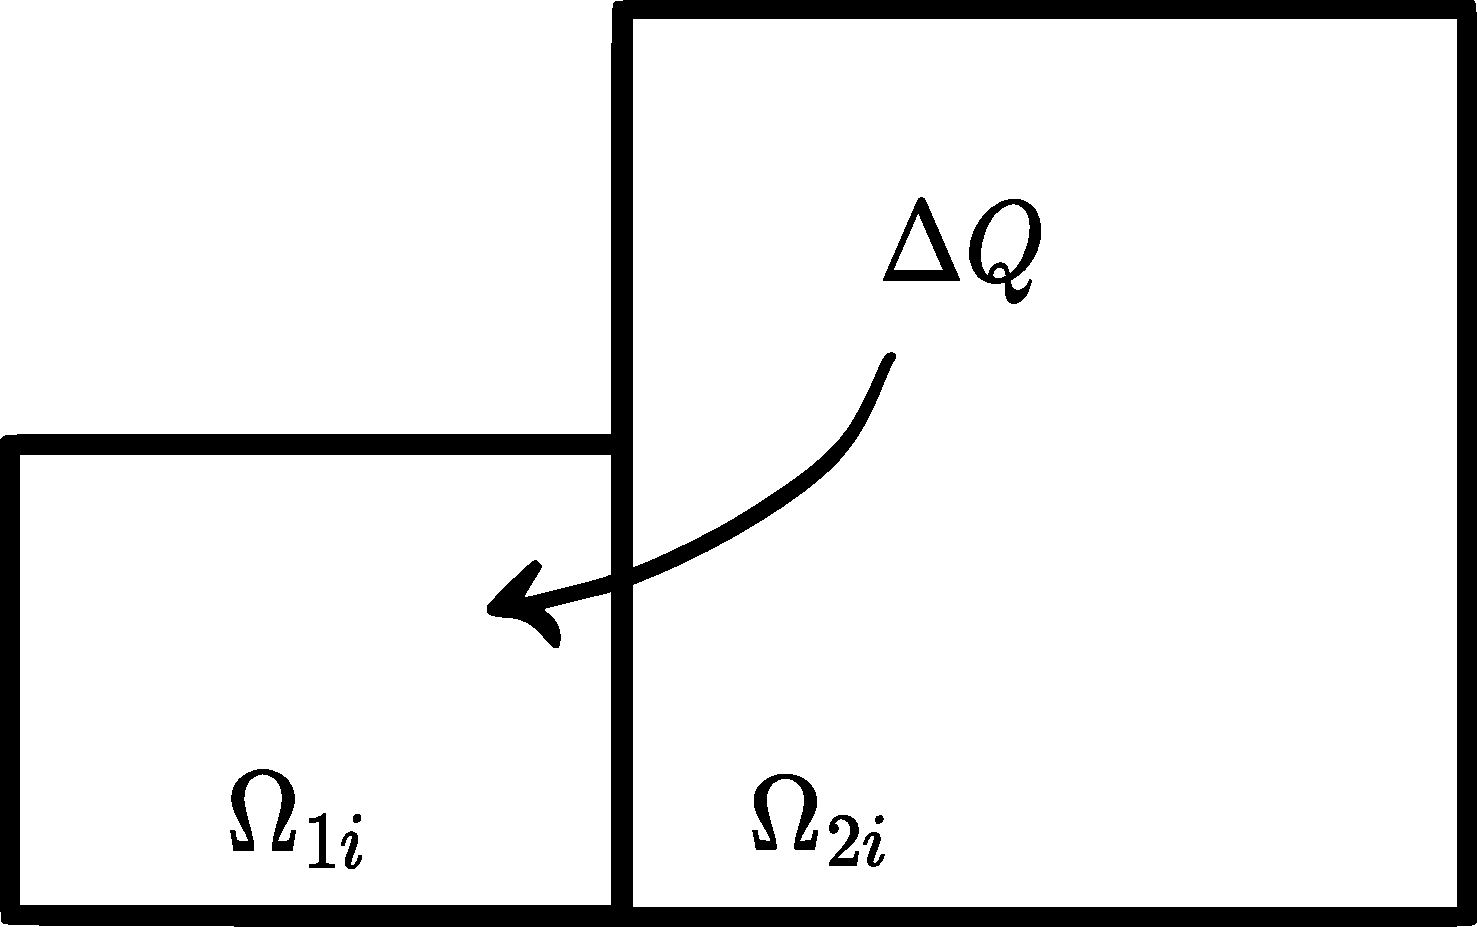
\includegraphics[scale=0.25]{fig/transf-calor.pdf}
\end{figure}

entonces hay $\Omega_{\text{tot},i}=\Omega_{1i}\cdot \Omega_{2i}$ estados accesibles al sistema combinado. Luego, la transferencia de calor ($\Delta Q$) hay $\Omega_{tot,f}=\Omega_{if}\cdot \Omega_{2f}$ estados accesibles al sistema combinado
\begin{equation}
  \Omega_{tot,f}>\Omega_{tot,i}
\end{equation}
En términos de la entropia:
\begin{equation}
  S_{1i}=k\log \Omega_{1i},\qquad  S_{2i}=k\log \Omega_{2i}
\end{equation}
Luego,
\begin{align}
  S_{tot,i}&=k\log \Omega_{tot,i}\\
  &=k\log (\Omega_{1i}\cdot \Omega_{2i})\\
  &=k\log (\Omega_{1i})+k\log (\Omega_{2i})
\end{align}
Así,
\begin{equation}
  S_{tot,i}=S_{1i}+S_{2i}
\end{equation}
Se concluye que la entropía es extensiva.

Notemos ademas que
\begin{equation}
  \Omega_{tot,f}>\Omega_{tot,i}\quad \Rightarrow \quad S_{tot,f}>S_{tot,i}
\end{equation}
es decir, la entropía aumenta en un proceso  de transferencia de calor.
\end{ej}

¿Cuál es la condición de equilibrio para que termine un proceso de transferencia de calor?

Cuando ambos sistemas quedan a la misma \textbf{temperatura}. Para definir temperatura, consideremos que en el nuevo equilibrio térmico:
\begin{equation}
  \left(\pdv{S_1}{U}\right)_{N,V}=-\left(\pdv{S_2}{U}\right)_{N,V}
\end{equation}
\begin{itemize}
	\item La energía interna $U$ cambia en ambos sistemas
	\item La ganancia $\Delta U_1$ en el sistema 1 es igual a la perdida $\Delta U_2$ en el sistema 2 (conservación de la energía).
	\begin{equation}
  \Delta U_1+\Delta U_2=0
\end{equation}
\item La entropía total aumenta, al cambiar $U$. Luego, $\Delta U$ deja de fluir cuando $S_{tot}$ deja de cambiar.
\item Se puede demostrar que el proceso continua hasta que (de lo anterior)
\begin{equation}
	\boxed{\left(\pdv{S_1}{U}\right)_{N,V}=-\left(\pdv{S_2}{U}\right)_{N,V}}
\end{equation}
\end{itemize}

Cuando
\begin{equation}
  \left(\pdv{S_1}{U}\right)_{N,V}=-\left(\pdv{S_2}{U}\right)_{N,V}
\end{equation}
entonces
\begin{equation}
  \left(\pdv{S_{tot}}{U}\right)_{N,V}=\left(\pdv{(S_1+S_2)}{U}\right)_{N,V}=\left(\pdv{S_1}{U}\right)_{N,V}+\left(\pdv{S_2}{U}\right)_{N,V}=0
\end{equation}
Luego,
\begin{equation}
\boxed{  \left(\pdv{S_{tot}}{U}\right)_{N,V}=0}
\end{equation}
y la entropía deja de aumentar con la transferencia de calor. Luego, el proceso se detiene. Así, conviene definir la temperatura $T$:
\begin{equation}
  \boxed{\frac{1}{T}=\left(\pdv{S}{U}\right)_{N,V}}\qquad \text{Al aumentar $T$ aumenta $U$.}
\end{equation}
Notamos que
\begin{equation}
  T_1=T_2\quad\Rightarrow\quad \frac{1}{T_1}=\frac{1}{T_2}\quad\Rightarrow \quad\left(\pdv{S_1}{U}\right)_{N,V}=\left(\pdv{S_2}{U}\right)_{N,V}
\end{equation}

\begin{cor}
	La transferencia de calor ocurre por gradiente de temperatura (el calor fluye desde e sistema de mayor temperatura hacia el de menor temperatura, asta que las temperaturas sean iguales).
\end{cor}

\subsection{Probabilidad de una configuración y factor de Boltzmann}
De la definición clásica de probabilidad, se tiene
\begin{equation}
  P=\frac{\# \text{casos favorables}}{\# \text{casos posibles}}
\end{equation}
El cuociente entre la probabilidad de dos estados macroscópicos es igual al cociente de sus \textit{degeneraciones.}

Considere un sistema "pequeño" de 2 estados, $S_p$ y un sistema "grande" o reservorio térmico $S_r$. Sea $U_0$ la energía del sistema combinado y $U_p$ la energía del sistema pequeño. Suponga que la energía del sistema $U_p$ puede ser $U_p=\epsilon$ y $U_p=0$.
\begin{itemize}
	\item Para $U_p=0$,\quad $U_r=U_0$\quad ($U_r$ energía del reservorio térmico)
	\item Para $U_p=\epsilon$,\quad $U_r=U_0-\epsilon$
\end{itemize}
El cociente entre las probabilidades esta dado por
\begin{equation}\label{1.1}
  \frac{P(\epsilon)}{P(0)}=\frac{\Omega(U_0-\epsilon)}{\Omega(U_0)}=\frac{e^{\frac{S}{k}(U_0-\epsilon)}}{e^{\frac{S}{k}(U_0)}}=\frac{\text{Prob. del $S_p$ con energía $\epsilon$}}{\text{Prob. del $S_p$ con energía $0$}}
\end{equation}
Luego, $\Omega(U)$ es la degeneración del reservorio térmico con energía $U$.

Expandiendo en serie de Taylor 
\begin{equation}
  S(U_0-\epsilon)\approx S(U_0)-\epsilon\left(\pdv{S}{U_0}\right)=S(U_0)-\frac{\epsilon}{T}
\end{equation}
Reemplazando en la exponencial de \eqref{1.1},
\begin{equation}
  \boxed{\frac{P(\epsilon)}{P(0)}\approx e^{-\frac{\epsilon}{kT}}}
\end{equation}
Conocido como el \textbf{factor de Boltzmann}.

La probabilidad relativa entre 2 estados escala como la exponencial de menos la diferencia de energía dividida por $kT$.

\begin{equation}
  \textbf{Mientras más energético un estado, menos probable.}
\end{equation}
































